\documentclass{beamer}

\mode<presentation> {
\usetheme{AnnArbor}
}

\usepackage{graphicx}
\graphicspath{{./figures/}}
\usepackage{caption}
\usepackage{subcaption}
\usepackage{hyperref}
\hypersetup{colorlinks=true}
\usepackage{amsmath}
\usepackage{amsthm}
%\usepackage[shortlabels]{enumitem}
\usepackage{biblatex}
\addbibresource{bibliography.bib}

\newtheorem{proposition}{Proposition}

\title[Statistical Methods for Extremal Events]{Statistical Methods for Extremal Events}

\author{Victor Verma}
\institute[]
{
Prof. Yang Chen's Reading Group \\
Department of Statistics \\
University of Michigan
}
\date[2/23/23]{2/23/23}

\begin{document}

\begin{frame}
    \titlepage
\end{frame}

\begin{frame}{Today's Reading}
    \begin{itemize}
        \item Chapter 6 of \textit{Modelling Extremal Events} by Embrechts, Kl\"{u}ppelberg, and Mikosch (\cite{embrechts_et_al_1997})
    \end{itemize}
\end{frame}

\begin{frame}{Outline}
    \tableofcontents
\end{frame}

\section{Graphical Methods}

\begin{frame}{Q-Q Plots}
    The motivating question: \textit{Find a df F which is a good model for the iid data $X, X_1, \ldots, X_n$}.

    \medskip

    Suppose that $X_1, \ldots, X_n \sim G(x) = F\left(\frac{x - \mu}{\sigma}\right)$ for some continuous df $F$, some $\mu \in \mathbb{R}$, and some $\sigma > 0$. Let $X_{n, n} \le \ldots \le X_{1, n}$ be the order statistics of the sample and let $G_n$ be the empirical df.

    \medskip

    Using the probability integral transform, $U_i = G(X_i) \sim \text{Uniform}(0, 1)$. Moreover,
    \[
    (G(X_{k, n})_{k = 1, \ldots, n} \overset{d}{=} (U_{k, n})_{k = 1, \ldots, n}.
    \]
    Since $U_{k, n}$ has pdf $\frac{n!}{(n - k)!(k - 1)!}u^{n - k}(1 - u)^{k - 1}I_{(0, 1)}(u)$ \cite{casella_and_berger_2002},
    \[
    E[G(X_{k, n})] = E(U_{k, n}) = \frac{n - k + 1}{n + 1}.
    \]
\end{frame}

\begin{frame}{Q-Q Plots}
    Thus, for large $n$,
    \[
    X_{k, n} = G_n^{\leftarrow}\left(\frac{n - k + 1}{n}\right) \approx G^{\leftarrow}\left(\frac{n - k + 1}{n + 1}\right) = \sigma F^{\leftarrow}\left(\frac{n - k + 1}{n + 1}\right) + \mu,
    \]
    so the graph
    \[
    \left\{\left(F^{\leftarrow}\left(\frac{n - k + 1}{n + 1}\right), X_{k, n}\right) : k = 1, \ldots, n\right\}
    \]
    should look linear.

    \smallskip

    This graph is a called a \textbf{Q-Q (quantile-quantile)} plot.
\end{frame}

\begin{frame}{Q-Q Plots}
    \begin{figure}
        \centering
        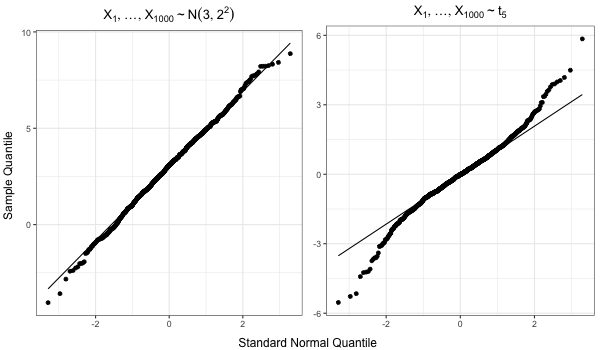
\includegraphics[scale=0.5]{qq_plots.png}
        \caption{Example Q-Q plots.}
        \label{fig:qq_plots}
    \end{figure}
\end{frame}

\begin{frame}{Q-Q Plots}
    Things we can do with Q-Q plots:
    \begin{enumerate}
        \item Check whether a proposed distribution for $X, X_1, \ldots, X_n$ is plausible
        \item Check for outliers
        \item Estimate location and scale parameters
        \item Compare shapes of distributions
    \end{enumerate}
\end{frame}

\begin{frame}{Q-Q Plots}
    Recall that a GEV (generalized extreme value) distribution $H_{\xi; \mu, \psi}$ satisfies
    \begin{align*}
        H_{\xi; \mu, \psi}(x) &= \exp\left\{-\left(1 + \xi\frac{x - \mu}{\psi}\right)^{-1 / \xi}\right\}, \quad 1 + \xi(x - \mu) / \psi > 0 \\
        &=
        \begin{cases}
            \Phi_{\alpha}\left(1 + \frac{x - \mu}{\alpha\psi}\right), & x > \mu - \psi\alpha, \ \xi = 1 / \alpha > 0 \\
            \Psi_{\alpha}\left(-\left(1 - \frac{x - \mu}{\alpha\psi}\right)\right), & x < \mu + \psi\alpha, \ \xi = -1 / \alpha < 0 \\
            \Lambda\left(\frac{x - \mu}{\psi}\right), & x \in \mathbb{R}, \ \xi = 0
        \end{cases}
    \end{align*}
    where
    \begin{align*}
        \text{(Fr\'{e}chet)} \quad \Phi_{\alpha}(x) &= \exp\left\{-x^{-\alpha}\right\}I_{(0, \infty)}(x) \\
        \text{(Weibull)} \quad \Psi_{\alpha}(x) &= \exp\{-(-x)^{\alpha}\}I_{(-\infty, 0)}(x) + I_{[0, \infty)}(x) \\
        \text{(Gumbel)} \quad \Lambda(x) &= \exp\left\{-e^{-x}\right\}
    \end{align*}
\end{frame}

\begin{frame}{Q-Q Plots}
    The GEV family isn't a location-scale family, but it has location-scale subfamilies. A strategy for making a Q-Q plot in the GEV case:
    \begin{enumerate}
        \item Compute an estimate $\hat{\xi}$ of $\xi$ (more on this later).
        \item Make a Q-Q plot with $X_1, \ldots, X_n$ and $H_{\hat{\xi}; 0, 1}$
    \end{enumerate}
    From the Q-Q plot, estimates $\hat{\mu}$ of $\mu$ and $\hat{\psi}$ of $\psi$ can be computed. $\hat{\xi}$, $\hat{\mu}$, and $\hat{\psi}$ can be used as initial values in a numerical procedure for obtaining more accurate estimates.
\end{frame}

\section{References}

\begin{frame}{References}
    \nocite{*}
    \printbibliography
\end{frame}

\end{document}